\documentclass[12pt]{article}
\usepackage[top=1.0in, bottom=0.6in, left=0.9in, right=1.1in]{geometry}

\usepackage{graphicx,color,enumitem}
\usepackage{amsmath,amsthm,amsbsy}
\usepackage{palatino}

\usepackage{tikz}

%% Setup aproblem environment, 
%% aproblem items
%% subproblems environment
%% subproblem items
\makeatletter
\newcounter{probcount}
\newcounter{subprobcount}
\newlength\probsep
\newlength\pshrinking
\newif\iffirstprob

\newenvironment{aproblems}%
  {\ifhmode\unskip\par\fi\setcounter{probcount}{0}\probsep\parskip
  \sbox\@tempboxa{\textbf{9.}}\pshrinking\wd\@tempboxa\advance\pshrinking\labelsep
  \let\hproblem\aproblem
  \advance\linewidth -\pshrinking
  \advance\@totalleftmargin\pshrinking
  \advance\leftskip\pshrinking}%
  {\ifhmode\unskip \par\fi\advance\leftskip-\pshrinking}%

\newcommand{\aproblem}{%
  \setcounter{subprobcount}{0}%
  \stepcounter{probcount}%
  \def\@currentlabel{\arabic{probcount}}%
  \ifhmode
    \unskip \par
  \fi
%  \addpenalty{-4000}%
  \iffirstprob\else\addvspace\probsep\fi
  \firstprobfalse
  \hskip -\labelwidth\hskip -\labelsep 
  \hbox to\labelwidth{\hss\textbf{\arabic{probcount}.}}\hskip\labelsep
}%

\newcommand{\subprob}{\item\def\@currentlabel{\arabic{probcount}\alph{\thelistlabel}}}
\newcommand{\skipproblem}{\stepcounter{probcount}}


%% The following commands put defined left and right headers on the top, and a page number
%% on the bottom of all pages beyond page 1
\usepackage{fancyhdr}
\pagestyle{fancy}
\fancyfoot[C]{\ifnum \value{page} > 1\relax\thepage\fi}
\fancyhead[L]{\ifx\@doclabel\@empty\else\@doclabel\fi}
\fancyhead[R]{\ifx\@docdate\@empty\else\@docdate\fi}
\headheight 15pt
\def\doclabel#1{\gdef\@doclabel{#1}}
\def\docdate#1{\gdef\@docdate{#1}}
\makeatother

%% General formatting parameters
\parindent 0pt
\parskip 6pt plus 1pt

\newcommand{\epart}[1]{\noindent \textbf{(#1)} \,}
\newcommand{\ds}{\displaystyle}

\doclabel{Math F302 Worksheet}
\docdate{10 November 2023}


\begin{document}
\renewcommand{\d}{\displaystyle}

\centerline{{\Large \textsc{Solving differential equations} \hspace{30mm}}}

\medskip
\centerline{{\Large \textsc{by series (\S6.2)} \hspace{33mm}}}

\vspace{-20mm}

\def\BEAVER{}
%\def\MOOSE{}
%\def\TURTLE{}

\ifdefined\BEAVER
\hfill 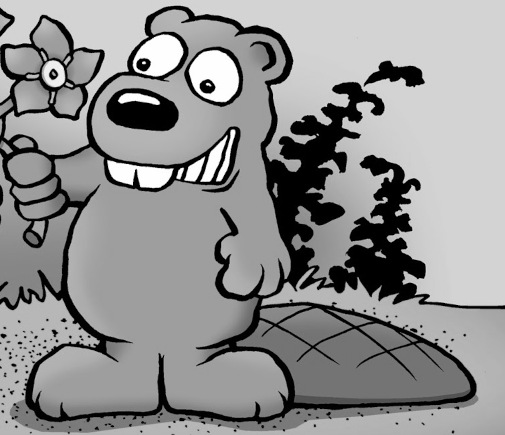
\includegraphics[height=30mm]{figs/beaver.jpg}
\else
\ifdefined\MOOSE
\hfill 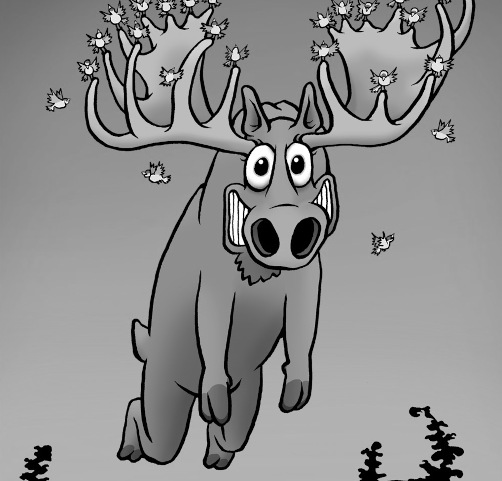
\includegraphics[height=30mm]{figs/moose.jpg}
\else
\hfill 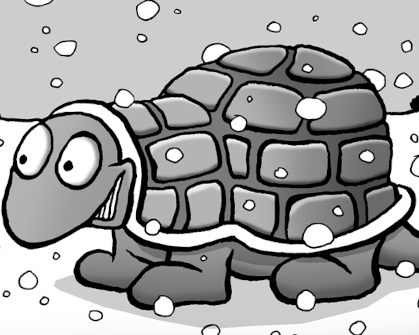
\includegraphics[height=30mm]{figs/turtle.jpg}
\fi
\fi

\vspace{-10mm}
\noindent
\fbox{
{\footnotesize
Team effort!  Find at least the first \emph{five} coefficients ($c_0,c_1,c_2,c_3,c_4$).}
}

\medskip
\ifdefined\BEAVER
\noindent Find the solution of the ODE IVP by an appropriate power series:
    $$y' + (x-1) y = 3, \quad y(1) = 2$$
\else
\ifdefined\MOOSE
\noindent Use the power series method to solve the initial value problem:
    $$(x+1) y'' + y = 0, \quad y(0)=0, \, y'(0)=1$$
\else
\noindent Use the power series method to solve the initial value problem:
    $$y'' + (x+1)  y = 0, \quad y(0)=1, \, y'(0)=0$$
\fi
\fi
\vfill
\end{document}
